\chapter{Technical Background} \label{chap: page-cache}
In this chapter we review the technical background that is required to understand the material treated in the first part of the thesis. We start by introducing the general idea
of file caching; afterwards, we describe the Linux kernel I/O architecture and more specifically the \textit{Page Cache} component that provides the file caching infrastructure in Linux; 
we conclude the chapter by reviewing the I/O hints interfaces provided by the Linux kernel and the GPFS filesystem, \textit{posix\_fadvise} and \textit{gpfs\_fcntl} respectively.

\section{Introduction to File Caching} \label{sec: gen-concept}
Information in a computer is persistently stored using files. A File is a data container organized as sequence of blocks. These blocks typically reside on a storage block device like a hard disk drive. 
A filesystem is a component of the operating system that provides user programs with all the functionalities they need to interact with files and manipulate them. The filesystem takes into account 
the geometry of the storage medium used to ultimately store the information, most commonly a magnetic disk in hard disks, and tries its best to make efficient use of it. For example, data blocks from 
the same file are placed close to each other on the magnetic disk because in this way it is possible to access all the data with a single hardware operation. If data is scattered all over the disk however, 
there will be several hardware operations involved to reposition the HDD head, i.e. the hard disk component that performs the physical reading and writing of data onto the storage medium, at the appropriate 
location (we will give more informations about hard disk drives in the rest of this section). Moving the HDD head on the disk plate is called \textit{seeking} and is a time consuming operation. Since accessing 
data from storage devices is a very slow process compared to accessing data from main memory, a file cache is employed to keep frequently requested file data in fast RAM. In this way a following request for 
the same data can be served more quickly from main memory, instead of a slow device. Caching in general exploits the physical characteristics of memory components in the system. Memory components are classified 
according to the scheme in Figure~\ref{figure: mem-hierarchy}, also called memory hierarchy. Memory components at the top of the pyramid, e.g. CPU registers, have lower latency and capacity compared to memory 
components at the bottom of the pyramid, e.g. hard disks, this is reflected on the higher cost per byte. Because the installation of large amounts of fast memory in the system is not economically feasible, 
different levels of caching are needed to hide the time penalties associated with data I/O to the memory components located at the bottom of the pyramid.

\begin{figure}[!htb]
  \centering
  \includegraphics[width=0.8\textwidth]{chapters/figures/mem-hierarchy}
  \caption{Typical memory hierarchy arrangement in modern computer systems. At the top of the pyramid we have low-latency, low-capacity memory components, while at the 
  bottom we have high-latency, high-capacity memory components. Cost per byte increases as we move towards the top and decreases as we move towards the bottom.}
  \label{figure: mem-hierarchy}
\end{figure}

In order to understand how a file cache works, we now look at how the operating system handles read and write operations generated by user applications. When the operating system receives
a read request for a file, it first looks for the requested data in the file cache. If the data is in the cache, also called \textit{cache hit}, it is copied to the provided user buffer and 
the control is returned to the application. If the data is not in the cache, also called \textit{cache miss}, the filesystem retrieves it from the storage device and places it in the cache. 

Write operations are handled differently. In particular, when the operating system receives a write operation it first writes the data to the cache, unless the program explicitly asks to write 
directly to the storage device using a mechanism called direct I/O. Data in the cache can be then copied to the storage device either in a blocking fashion, meaning that the operating system 
does not return control to the program until data is safe in the storage hardware, or in a non blocking fashion, meaning that the operating system immediately returns control to the program 
and copies the data to the storage device later on. The blocking approach is called \textit{write-through}, while the non-blocking approach is called \textit{write-back}.

Since data from the same file is typically arranged contiguously in the block device hardware, the filesystem can exploit this spatial locality to bring into the cache more data than requested,
making the assumption that contiguous data has a high chance of being requested in the future. This process is called \text{prefetching} and is at the base of the optimizations proposed in 
the first part of this thesis. Prefetching is carried out using a technique called read-ahead. As the name suggests, upon receiving a read request for a certain file range, the filesystem 
brings into the cache the requested data plus a certain amount of adjacent data that follows it in the file. If the guess is correct, future requests will generate a cache hit and  the file 
system keeps performing read-ahead by increasing the amount of data prefetched for future requests. On the other hand, if the guess is wrong future requests will generate a cache miss and 
valuable cache space is wasted.

Because the amount of physical memory is limited, when available memory capacity goes low the filesystem needs to decide what data can be removed from the cache to accommodate new data. This 
process is called \textit{eviction} and can be performed using different policies. One example is the First In First Out (FIFO) policy, in which data that was first placed in the cache is 
removed first. Another more effective and adopted policy is the Last Recently Used (LRU), in which the last accessed data in the cache is removed first. This locality mechanism works pretty 
well because programs are cyclic by nature, they periodically access the same instruction and information in order to perform some recursive task.

\section{Introduction to the Linux Kernel} \label{sec:kern-arch}
The Linux kernel is the core component of many different operating systems, also called Linux derivatives for this reason. Since user programs typically are not allowed to interact directly
with the system hardware, the kernel provides a set of basic functionalities for this. One immediate advantage of such separation is that the kernel can hide low-level hardware details to 
users and present them a simpler view, or abstraction, of the system that they can use to perform their tasks. In this way only the kernel programmer needs to understand how the 
hardware works. In fact, Linux uses abstractions at many different levels in its architecture. For example, users in Linux have the illusion of being in control of all the memory in the system 
while in fact, they are restricted to access only a limited area of main memory called \textit{User Space} that is separated from the memory area used by kernel, called \textit{Kernel Space}. 
This abstraction is called virtual memory. Here we focus on the filesystem and I/O architecture. Figure~\ref{figure: io-arch} shows the components of the Linux kernel that are involved during 
I/O operations to storage devices, e.g. HDDs, as described by~\cite{Cesati}.

\begin{figure}[!htb]
  \centering
  \includegraphics[width=0.5\textwidth]{chapters/figures/io_architecture}
  \caption{Kernel components involved in a block device operation.}
  \label{figure: io-arch}
\end{figure}

\vspace{5mm}
\textbf{Hard Disks Drives} are the most used mechanical storage components for persistently storing data in a computer. Data in hard disks is organized into sectors (elementary storage units), 
dislocated on the surface of a magnetic disk (or platter). Hard disks can have many platters arranged into a stack connected through a spindle powered by an electrical motor. Data on the disk is 
accessed through sensors, or heads, that are moved over the disk surface to read and write data using a set of mechanically actuated arms. Sectors are further organized into tracks, i.e. concentric 
strips that can be accessed with a single head positioning (seek), the disk spins at high speed allowing the head to access all the sectors in the track. Finally the set of tracks, from the different 
platters, that are located at the same distance from the spindle is called cylinder. Since every platter is paired with a set of heads, one for the lower surface and one for the upper, data on the same
cylinder can be accessed at the same time using the available heads. Figure~\ref{figure: hdd} shows the described device geometry. Although hard disks can transfer data at the granularity of the 
sector, in order to achieve acceptable performance data is typically transfered into larger units containing multiple sectors. These units are called blocks and thus hard disks are also called block 
devices. Another feature of hard disks is that they allow data to be accessed in any order, making them another type of random access memory, similarly to RAM.

\begin{figure}[!htb]
  \centering
  \includegraphics[width=0.8\textwidth]{chapters/figures/hdd}
  \caption{Schematic representation of the components of a hard disk drive.}
  \label{figure: hdd}
\end{figure}

\vspace{5mm}
\textbf{Block Device Drivers} are software modules that can be dynamically loaded and unloaded from the kernel. Device drivers are the lowest component in the Linux block system and provide a bridge
between the I/O scheduler and the hardware. More specifically, they convert block device requests into commands for the hardware. One fundamental characteristic of device drivers is that they are 
interrupt driven, that is, they do not run synchronously but instead asynchronously. This characteristic is exploited by the I/O scheduler to improve the performance of the block system.

\vspace{5mm}
\textbf{The I/O Scheduler} is an essential component for the good performance of I/O block device operations. To understand how the I/O scheduler improves I/O performance let's consider the example of 
a simple file open operation. A file in the filesystem is represented on disk by a data structure called \textit{inode} and is typically contained into a single filesystem block. The inode data structure 
contains the mapping between logical blocks in the file and physical blocks in the device. The file open operation in our example, is serviced by the kernel by creating a new block device request for the 
block containing the inode and then invoking the I/O scheduler to schedule it. Nevertheless, the request is not satisfied immediately by the block device driver but is delayed to a later time. Servicing 
the request immediately would prevent the kernel from looking at multiple requests at the same time, missing the opportunity for merging them and reducing the actual number of physical operations involved 
in the I/O operation. Indeed, upon receiving a new request from the generic block layer, the I/O scheduler tries to understand if it can be serviced by enlarging a preexisting request. If this is possible 
two separate requests will be merged into a single one. 

\vspace{5mm}
\textbf{The Generic Block Layer} is a kernel component that manages all the block devices in the system. It provides a representation of the block devices as a linear arrangement of logical blocks
to the filesystem. This allows the generic block layer to aggregate blocks from different physical devices and present them as a unique block device (or virtual block device). This powerful abstraction
is exploited by volume manager softwares such as LVM. The main data structure used by the generic block layer is the \texttt{bio} structure. Every I/O block device operation in the system is described 
by a bio instance. The bio contains information such as the initial sector number and the number of sectors to be transfered for the request. Additionally, the bio contains a set of references to the 
memory areas that are involved in the I/O operation. The memory area references are used by the hard disk controller to transfer data through Direct Memory Access (DMA) operations, relieving the CPU 
from spending time in slow data transfer operations.

\vspace{5mm}
\textbf{The Filesystem} component provides the mapping layer allowing the operating system to locate logical blocks of the file in the physical block device. The native filesystem in Linux is the Second 
Extended Filesystem (Ext2).

\vspace{5mm}
\textbf{The Page Cache}

\vspace{5mm}
\textbf{The Virtual File System}

\section{The Page Cache}
The page cache represents the primary disk cache in the kernel. It consists of physical pages in RAM, each composed by a certain number of blocks from the disk. These blocks can be distributed arbitrarily
in the file. For this reason every data block in the page is handled differently 

\section{The POSIX Advice API}
\label{sec: posix_advice_api}
The Linux kernel allows users to control page cache functionalities through the \texttt{posix\_fadvise()} system call: 
$$\textit{\textbf{int} posix\_fadvise(\textbf{int} fd, \textbf{off\_t} offset, \textbf{off\_t} len, \textbf{int} advice)}$$ 
This system call takes four input parameters: a valid file descriptor representing an open file, starting offset and length of the file region the advice will apply to, and finally the type 
of advice. The implementation provides five different types of advice, that reflect different aspects of caching.

\begin{table}[!htb]
\centering
\ra{1.5}
\caption{Values for \textit{advice} in the \textit{posix\_fadvise()} system call}
\newcolumntype{K}{>{\centering\arraybackslash} m{4cm}}
\newcolumntype{V}{>{\centering\arraybackslash} m{5cm}}
\begin{tabular}{KV}
\toprule
\bf \small Advice & \bf \small Description \\
\midrule
\small \ttfamily POSIX\_FADV\_SEQUENTIAL & \small file I/O pattern is sequential \\
\small \ttfamily POSIX\_FADV\_RANDOM & \small file I/O pattern is random \\
\small \ttfamily POSIX\_FADV\_NORMAL & \small reset file I/O pattern to normal \\
\small \ttfamily POSIX\_FADV\_WILLNEED & \small file range will be needed \\
\small \ttfamily POSIX\_FADV\_DONTNEED & \small file range won't be needed \\
\small \ttfamily POSIX\_FADV\_NOREUSE & \small file is read once (not implemented) \\
\bottomrule
\end{tabular}
\label{table: advice_table}
\end{table}

The first two advice in Table~\ref{table: advice_table} have an impact on spatial locality of elements of the cache. \texttt{POSIX\_FADV\_SEQUENTIAL} can be used to advise the kernel that a 
file will be accessed sequentially. As result the kernel will double the maximum read-ahead window size in order to have a greedier read-ahead algorithm. \texttt{POSIX\_FADV\_RANDOM}, on the 
other hand, can be used when a file is accessed randomly and has the effect of completely disabling read-ahead, therefore only ever reading the requested data. Finally, \texttt{POSIX\_FADV\_NORMAL} 
can be used to cancel the previous two advice-messages and reset the read-ahead algorithm to its defaults. These three advice types apply to the whole file, the offset and length parameters are 
ignored for these `modes'.

Two of the remaining three advice types have an impact on the temporal locality of cache elements. \texttt{POSIX\_FADV\_WILLNEED} can be used to advise the kernel that the defined file region will 
be accessed soon, and therefore the kernel should prefetch the data and make it available in the page cache. \texttt{POSIX\_FADV\_DONTNEED} has the opposite effect, making the kernel release the 
specified file region from the cache, on the condition that the corresponding pages are clean (dirty pages are not released). Finally, the implementation for \texttt{POSIX\_FADV\_NOREUSE} is not 
provided in the kernel.

One important aspect of \texttt{posix\_fadvise()} is that it is a synchronous system call. This means that every time an application invokes it, it blocks and returns only after the triggered read-ahead 
operations have completed. This represents a big limitation especially if we consider \texttt{POSIX\_FADV\_WILLNEED} that may need to prefetch an arbitrarily large chunk of data. In this scenario the 
application may be idle for a long period of time while the data is being retrieved by the filesystem.

\section{The GPFS Hints API}
\label{sec: gpfs_hints_api}
The GPFS filesystem is a POSIX I/O compliant distributed filesystem for large clusters. GPFS code runs in kernel context but does not rely on the page cache infrastructure provided by Linux to cache
file data. On the other hand GPFS defines its own page cache infrastructure that is kept in a separated area of main memory called page pool. Similarly to POSIX advice, GPFS provides users with the ability 
to control page pool functions through the \texttt{gpfs\_fcntl()} subroutine: 
$$\textit{\textbf{int} gpfs\_fcntl(\textbf{int} fileDesc, \textbf{void}* fcntlArgP)}$$ 
The subroutine takes two inputs: the file descriptor of the open file to which hints will be applied to, and a pointer to a data structure residing in the application's address space. The indicated data 
structure contains all the information regarding what hints should be sent to GPFS. Specific hints are described by means of additional data structures that are contained in the main struct. 
Table~\ref{table: hints_table} summarizes all the available hints data structures and reports the corresponding description for each of them.

\begin{table}[!htb]
\centering
\ra{1.5}
\caption{GPFS hint data structures}
\newcolumntype{K}{>{\centering\arraybackslash} m{4.5cm}}
\newcolumntype{V}{>{\centering\arraybackslash} m{6cm}}
\begin{tabular}{KV}
\toprule
\bf \small Hint data structure & \bf \small Description \\
\midrule
\small \ttfamily gpfsAccessRange\_t & \small defines a file range to be accessed \\
\small \ttfamily gpfsFreeRange\_t & \small defines a file range to be released \\
\small \ttfamily gpfsMultipleAccessRange\_t & \small defines multiple file ranges to be accessed \\
\small \ttfamily gpfsClearFileCache\_t & \small releases all the page pool buffers for a certain file \\
\bottomrule
\end{tabular}
\label{table: hints_table}
\end{table}

Hints are not mandatory and GPFS can decide to accept or ignore them depending on specific conditions. Consider, for example, the multiple access range hint as an example (\texttt{gpfsMultipleAccessRange\_t} 
in table~\ref{table: hints_table}). The data structure corresponding to this hint is reported in Listing~\ref{list: mar}. 

\begin{lstlisting}[language=C, caption=Multiple Access Range Hint Data Structure, label={list: mar}, basicstyle=\ttfamily\scriptsize]
define GPFS_MAX_RANGE_COUNT 8

typedef struct {
    long long blockNumber;
    int start;
    int length;
    int isWrite;
    char padding[4];
} gpfsRangeArray_t;

typedef struct {

   int structLen;
   int structType;
   int accRangeCnt;
   int relRangeCnt;
   gpfsRangeArray_t accRangeArray[GPFS_MAX_RANGE_COUNT];
   gpfsRangeArray_t relRangeArray[GPFS_MAX_RANGE_COUNT];

} gpfsMultipleAccessRange_t;

\end{lstlisting}

The multiple access range data structure contains two sets of parameters, one set describing what filesystem blocks should be placed in the GPFS page pool and one set describing what filesystem blocks are 
no longer needed and should therefore be removed from the page pool. The \texttt{accRangeCnt} integer defines the number of blocks requested using the array \texttt{accRangeArray}, while \texttt{relRangeCnt} defines 
the number of blocks that should be evicted using the array \texttt{relRangeArray}. Unlike POSIX advice, in which the user does not need to explicitly evict cached blocks from the page cache, in GPFS users have 
to manually handle the release of blocks in the page pool. If this is not done the filesystem will stop accepting new access hints which are thus ignored. As we will see in the next chapter, Mercury transparently
handles the release of unused blocks for the user based on the I/O pattern description provided by the user itself.

%
%texttt{gpfsMultipleAccessRange\_t} contains two range arrays instead of just one: \texttt{accRangeArray}, used to define \texttt{accRangeCnt} blocks of the file that GPFS has to prefetch, and 
%texttt{relRangeArray} used to define \texttt{relRangeCnt} blocks of the file previously requested using \texttt{accRangeArray} and that are no longer needed. Unlike posix\_fadvise the user has to manage 
%he list of blocks for which hints have been sent, updating whether they are still needed. Indeed, if the accessed blocks are not released, GPFS will stop accepting new hints once the maximum internal number 
%f prefetch requests has been reached. 
%
%begin{lstlisting}[language=C, caption=Multiple Access Range Hint Initialisation and Submission, label={list: mar_example}, basicstyle=\ttfamily\scriptsize]
%oid mercury::BlockCache::gpfsAccessReleaseBlock(
%   std::vector<mercury::block_t>& access, 
%   std::vector<mercury::block_t>& release)
%
% struct
% {
%   gpfsFcntlHeader_t hdr;
%   gpfsMultipleAccessRange_t marh;
% } accHint;
%
% accHint.hdr.totalLength = sizeof(accHint);
% accHint.hdr.fcntlVersion = GPFS_FCNTL_CURRENT_VERSION;
% accHint.hdr.fcntlReserved = 0;
% accHint.marh.structLen = sizeof(accHint.marh);
% accHint.marh.structType = GPFS_MULTIPLE_ACCESS_RANGE;
% accHint.marh.accRangeCnt = access.size();
% accHint.marh.relRangeCnt = release.size();
%
% for (i = 0; i < accHint.marh.accRangeCnt && 
%     i < GPFS_MAX_RANGE_COUNT; i++)
% {
%   accHint.marh.accRangeArray[i].blockNumber = 
%     access[i].blockNumber_;
%   accHint.marh.accRangeArray[i].start = 
%     access[i].startOffset_;
%   accHint.marh.accRangeArray[i].length = 
%     access[i].blkLen_;
%   accHint.marh.accRangeArray[i].isWrite = 
%     access[i].isWrite_;
% }
% for (i = 0; i < accHint.marh.relRangeCnt && 
%     i < GPFS_MAX_RANGE_COUNT; i++)
% {
%   accHint.marh.relRangeArray[i].blockNumber = 
%     release[i].blockNumber_;
%   accHint.marh.relRangeArray[i].start = 
%     release[i].startOffset_;
%   accHint.marh.relRangeArray[i].length = 
%     release[i].blkLen_;
%   accHint.marh.relRangeArray[i].isWrite = 
%     release[i].isWrite_;
% }
%
% /* issue the hints to gpfs */
% if (gpfs_fcntl(fd_, &accHint))
% {
%   std::cerr << "gpfs_fcntl access hint failed for " <<
%     fd_ << " errno=" << errno << " errorOffset=" <<
%     accHint.hdr.errorOffset << std::endl;
%   exit(EXIT_FAILURE);
% }
%
% /* remove the accessed and released blocks */
% access.erase(access.begin(), 
%   access.begin() + accHint.marh.accRangeCnt);
% release.erase(release.begin(), 
%   release.begin() + accHint.marh.relRangeCnt);
%
%end{lstlisting}

%Listing~\ref{list: mar_example} shows an example for the multiple access range hint initialisation and submission. In the example the \codeword{gpfsAccessReleaseBlock()} function receives two vectors, each 
%containing a number of regions that have to be prefetched (\texttt{access}) and released (\texttt{release}). Every access and release region defines the block number the current request starts from (\texttt{blockNumber\_}), 
%the start offset inside the block (\texttt{startOffset\_}), the length of the block (\texttt{blkLen\_}) and if the request is a read or a write (\texttt{isWrite\_}). For every requested range the implementation fills the 
%\codeword{accRangeArray} and the \codeword{relRangeArray} and finally submits the data structure to \codeword{gpfs\_fcntl()} to be served.
